\section{Der Phasenübergangsautomat}

Damit der Schwarm ein koordiniertes Manöver ausführen kann, um einem Objekt auszuweichen, hat sich der
Autor für einen Phasenübergangsautomaten entschieden. Ein Phasenübergangsautomat (im Weiteren als PTM 
für Phase Transition Machine) wechselt ihren Zustand nur, wenn eine spezifische Nachricht von einem
Roboter den gesamten Schwarm erreicht hat. Da wir die verteilte Breitensuche als Kommunikationsmittel
verwenden wechselt der Automat also erst den Zustand, wenn ein Baum mit einer Nachricht aufgespannt wurde.\\

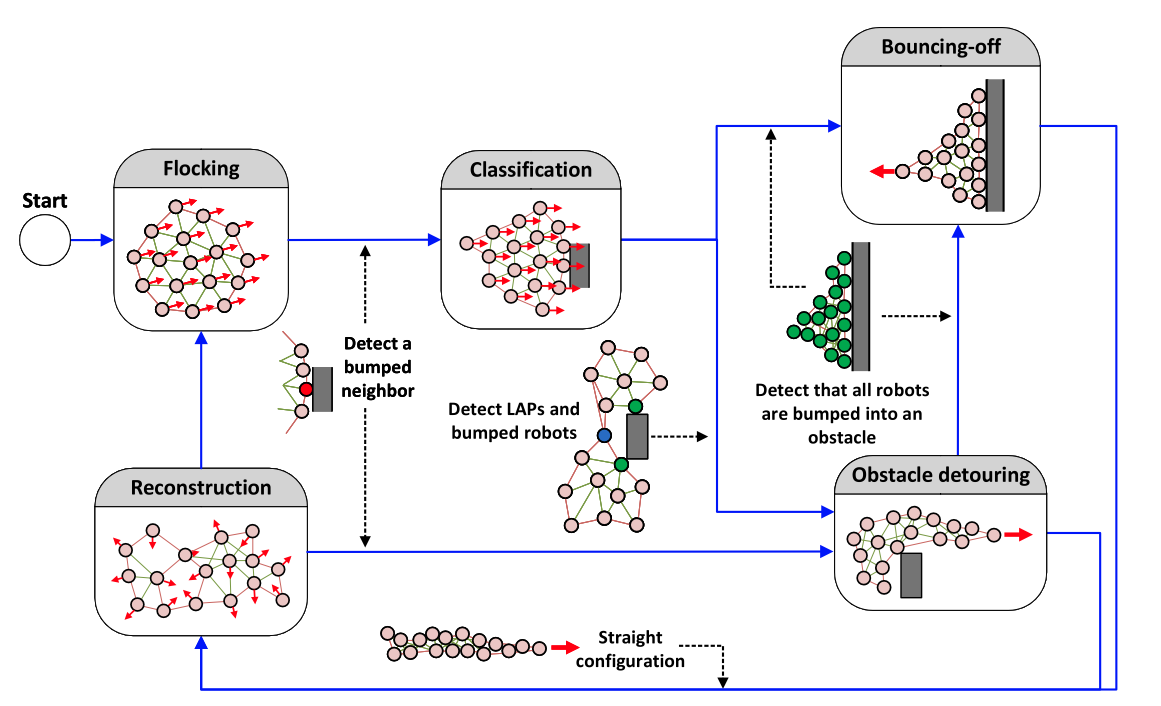
\includegraphics[width=5in]{images/Screenshot 2023-02-20 at 1.02.59 PM.png}